%% This is an example first chapter.  You should put chapter/appendix that you
%% write into a separate file, and add a line \include{yourfilename} to
%% main.tex, where `yourfilename.tex' is the name of the chapter/appendix file.
%% You can process specific files by typing their names in at the 
%% \files=
%% prompt when you run the file main.tex through LaTeX.

\singlespacing{

\chapter{Related Work}\label{chapter:RelatedWork}


The following sections outline current research into digital assembly across scales, CAD/simulation packages which occupy a similar space to what I propose, and programmable self assembly.

%An active area of synthetic biology explores the possibility of creating a viable cell from scratch based on knowledge about the core systems required for metabolism, cell maintainance, and self replication \cite{Forster2006}.  To date, efforts at creating this "minimal cell" have only been successful using a top down approach - starting with an organism with a minimal genome and reducing its genes further \cite{Glass2006} \cite{Gibson2010}.

\section{Programmable Materials}

The term "programmable matter" was first used to describe CAM8, a computing architecture in which physical phenomena could be efficiently simulated based on local interactions between parallel computing elements \cite{Toffoli1991}.  It has since come to describe materials that can be programmed to change their physical properties based on user input or environmental changes.  Often, programmable materials are composed of many smaller constituent elements, whose structural arrangement and local interactions are the source of larger-scale programmable properties.  Some forms of programmable material include metamaterials, modular robotics, 


the constituent elements that make up a piece of programmable matter do not have any inherient \\

Digital materials

\section{Digital Assembly}

Digital assembly is an emerging multimaterial fabrication technique where a finite set of discrete part types are (often reversibly) joined to form larger structures in a regular lattice.  Programmable functional behavior is achieved by patterning parts with different material properties across an assembly.  In the macro scale, the assembly process is orchestrated by one or many robotic assemblers.  Self-alignment features and the regular spacing of the parts help to minimize the complexity of a robotic assembler, and maintain global metrology through local interactions.  At nano scales, assembly is often guided by programmable self-assembly mechanisms.

\subsection{Macro Assembly}

Cheung showed that carbon fiber composite parts can be reversibly assembled to form ultralight materials for aerospace applications \cite{Cheung2013}.  Programmable flexibility is achieved by pattering rigid and flexural parts across an assembly and also by varying the density and connectivity of the parts.  Additional research into digital assembly of structural elements is ongoing at CBA, including modeling of the parts and assemblies using finite element analysis \cite{Calisch2014} and designing new part geometries and robotic assemblers \cite{Carney2015}.

\subsection{Micro Assembly}

\begin{figure}
  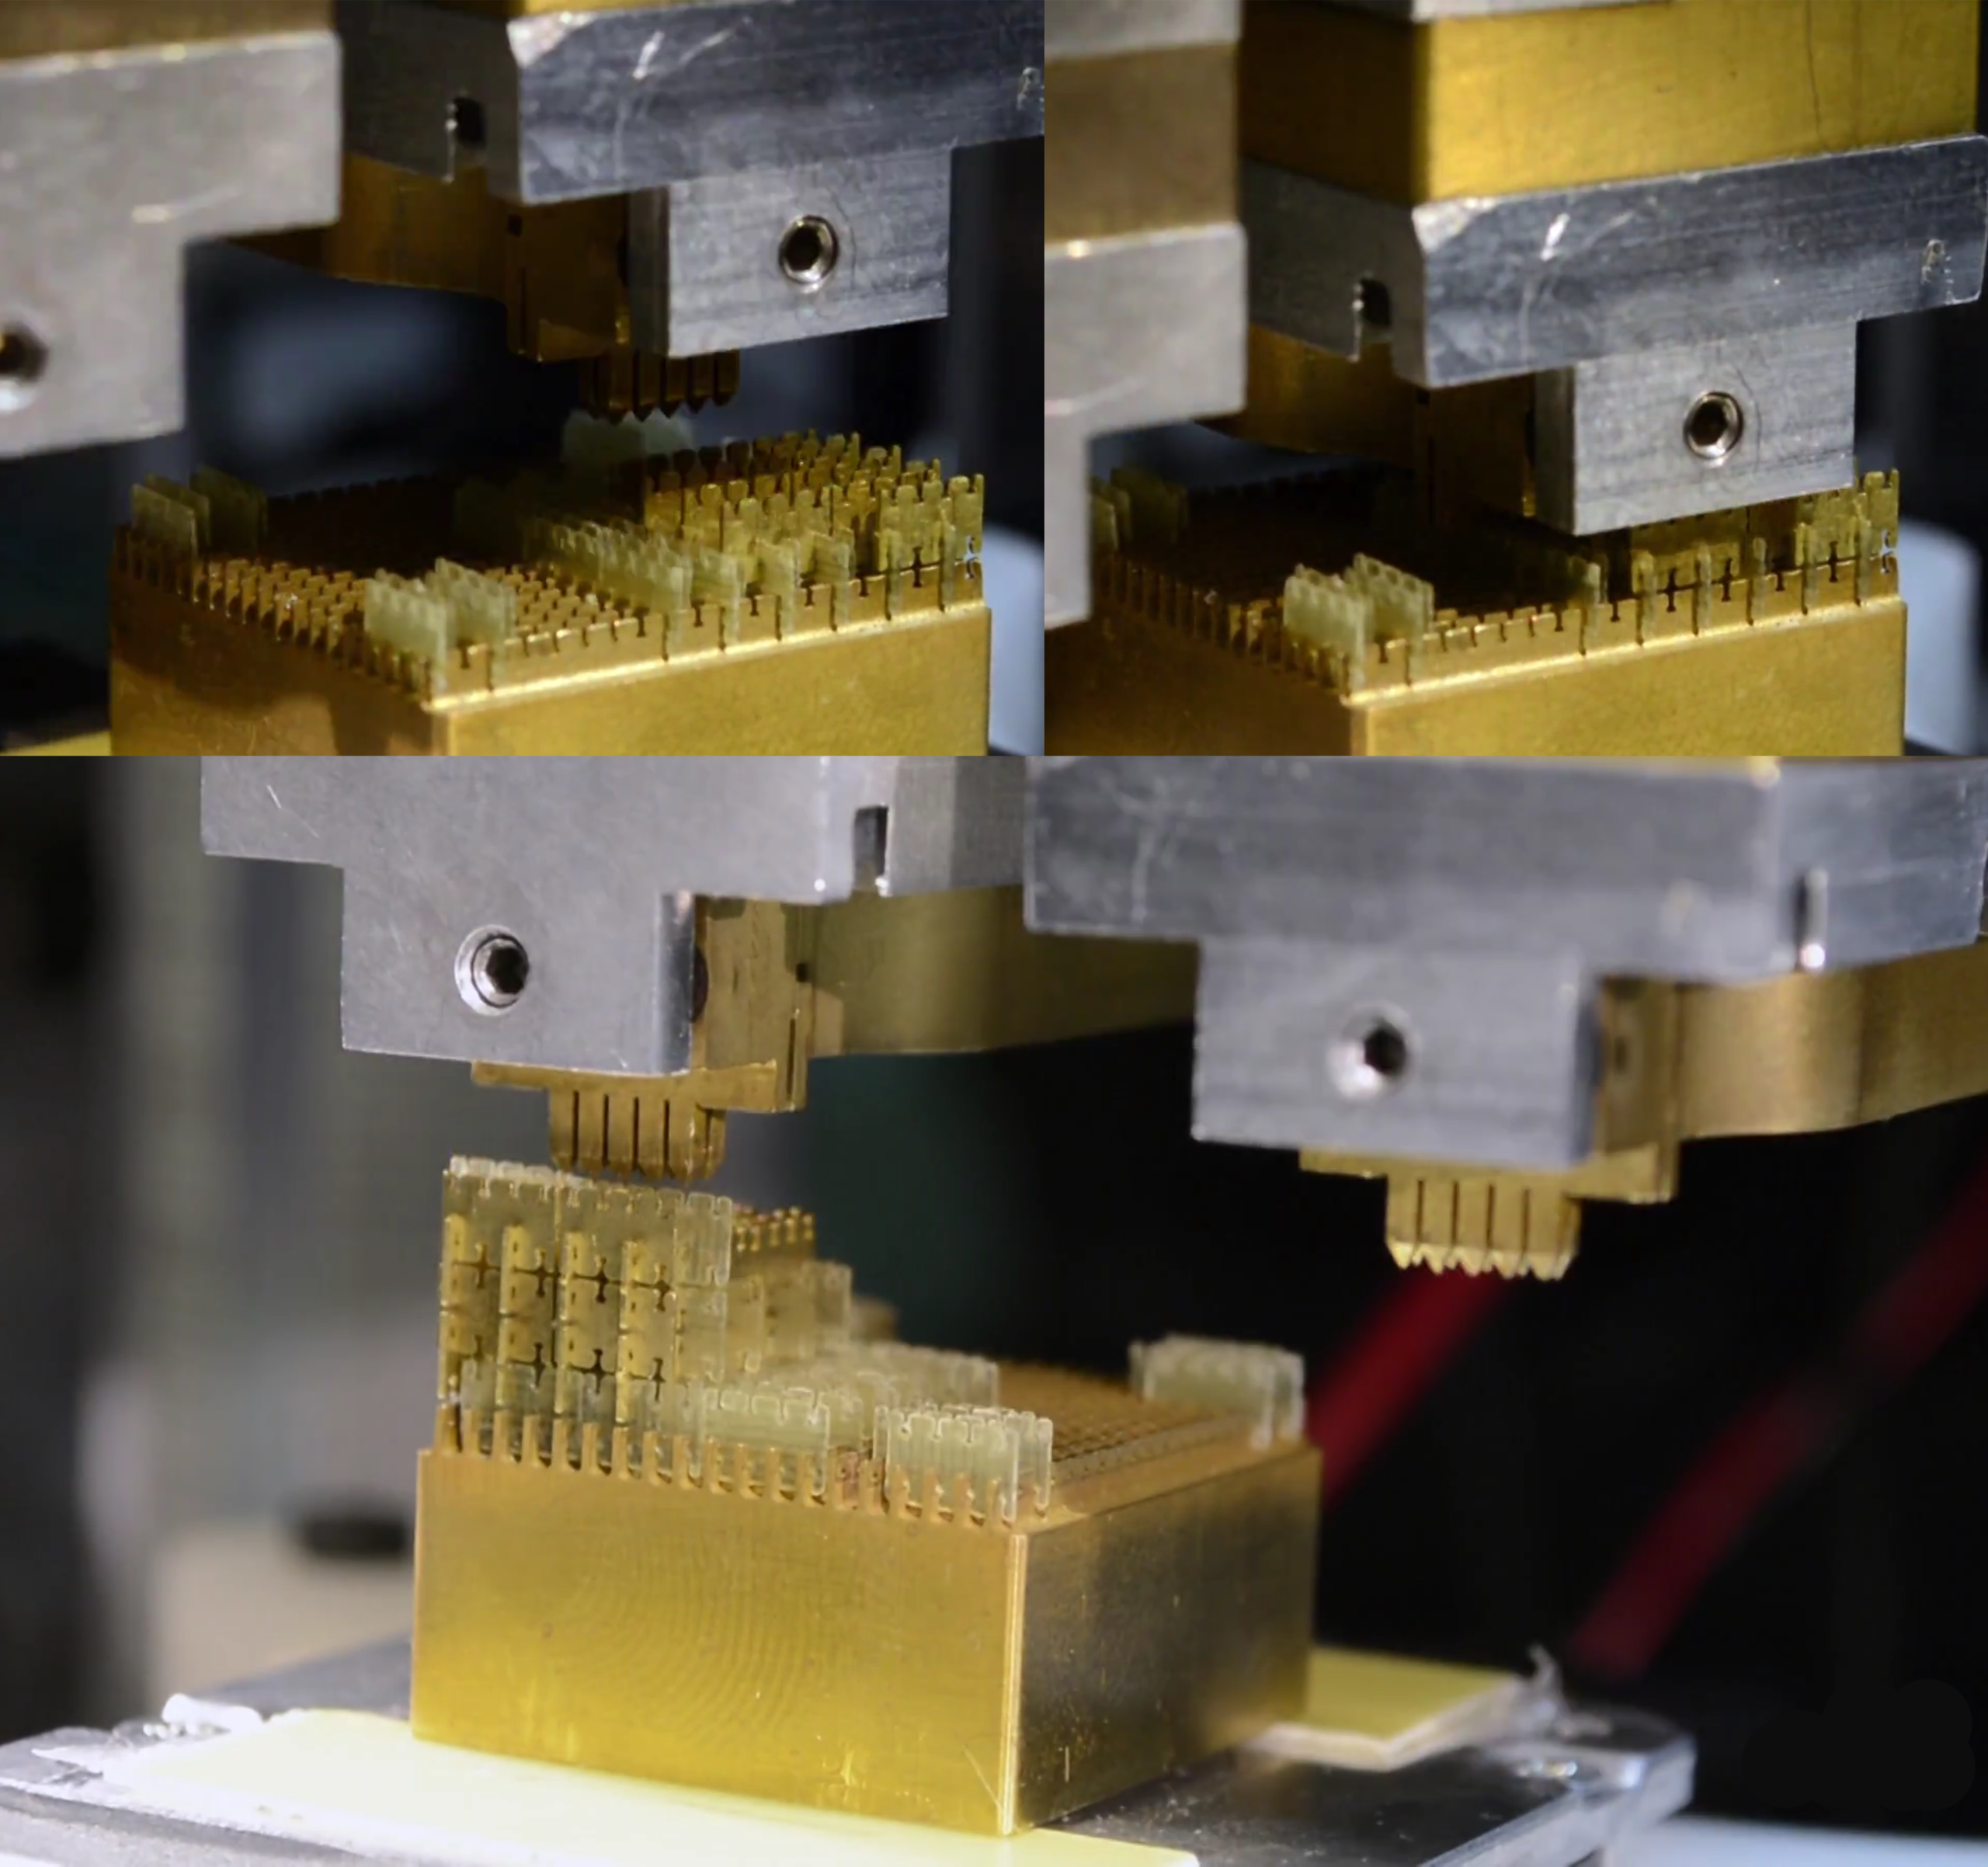
\includegraphics[width=\linewidth]{willAssembler.png}
  \caption{"Stapler" assembler designed by Will Langford assembles conductive and insulating discrete part types to form electronic structures with tunable capacitance and inductance.  \textit{Image Credit: Will Langford 2015}}
  \label{fig:willAssembler}
\end{figure}


%\begin{figure}
%  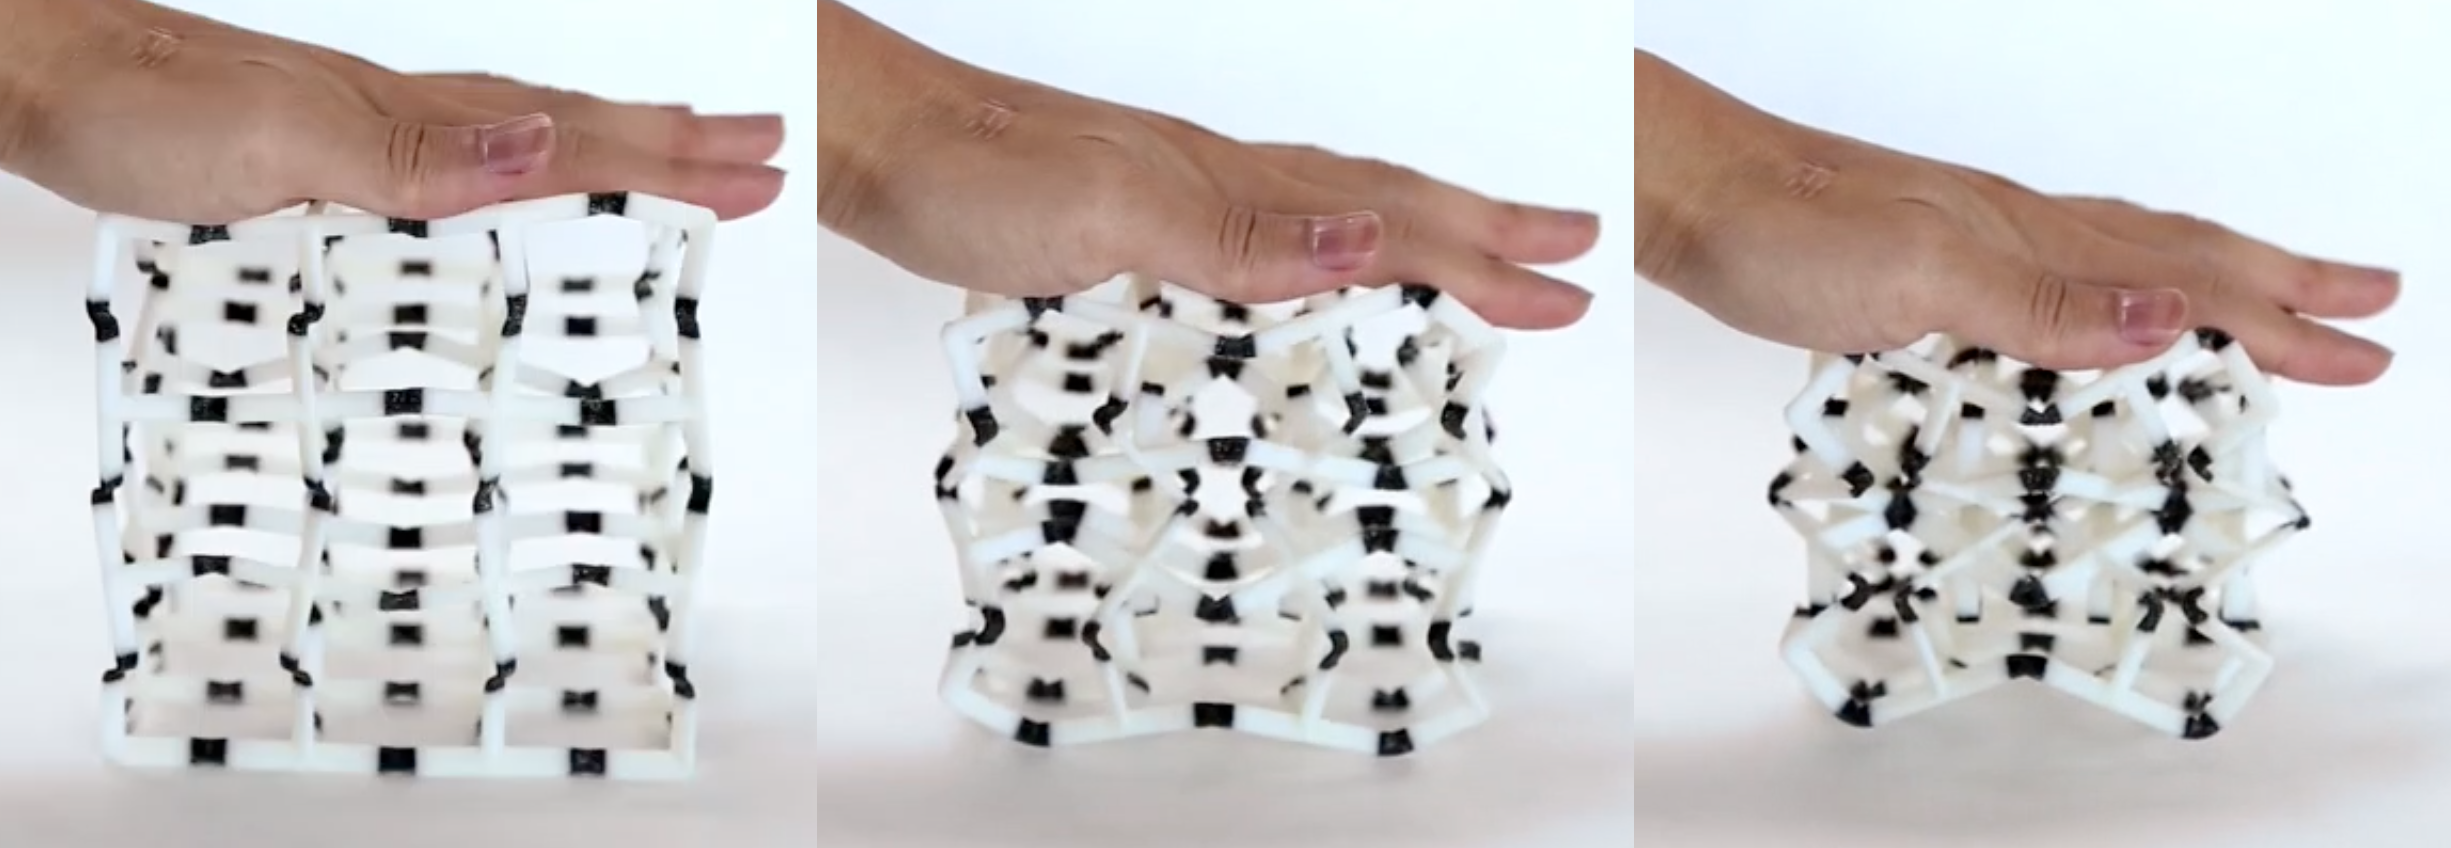
\includegraphics[width=\linewidth]{objetMultimaterial.png}
%  \caption{Mechanical properties programmed by material deposition in Objet 3D print.}
%  \label{fig: objetMultimaterial}
%\end{figure}

Langford demonstrated how conducting, insulating, and resistive part types ranging in scale from mm-$\mu$m could be assembled to form any passive electronic component, including antennas and RF matching networks \cite{Langford2014}.  Langford designed and built a dual-material assembler (Fig: \ref{fig:willAssembler}) for constructing passive electronic structures from conducting and insulating parts (\href{http://dma.cba.mit.edu/stapler/video/dualstapler_full_1.mp4}{video}) \cite{LangfordWillGhassaeiAmandaGershenfeld2016}.  Langford suggests that by extending the part types to include several types of silicon components, discretely-assembled active components like diodes and transistors would be possible.  Work toward the fabrication and realization of these silicon components is ongoing.  This work follows from previous work by Popescu et al. on reversibly assembled "GIK" structures spanning many length scales and material types \cite{Popescu} and also work by Ward on discretely assembled electronics \cite{Ward2010}.
\\

Hiller et al. propose a method of additive manufacturing using multimaterial voxel building blocks \cite{Hiller2009a}.  They explore various voxel decompositions of 3D geometry and assess their suitability for rapid, parallel assembly processes (\href{https://www.youtube.com/watch?v=-szjlhVMGh4}{video}).  Possible applications discussed include desktop manufacturing, especially for electromechanical and microfluidic devices.  Hiller et al. also propose reversible processes for disassembling voxel assemblies back into their constituent parts \cite{Hiller2005}.
\\

Though not a reversible process, multimaterial 3D printing (most notably by the Objet printer) deposits material in voxels on the order of ~10$\mu$m$^{3}$ with a total build volume on the order of 1x10$^{10}$ voxels \cite{Objet1000}.  Multimaterial 3d printing has been demonstrated in optical \cite{Willis2012}, electronic \cite{Ahn2009}, and structural applications \cite{Skouras2013} \cite{Schumacher} \cite{Bacher2014}.

\subsection{Nano Assembly}

"DNA bricks" is a method of discrete nano-assembly based on complementary base pair interactions of short segments of DNA \cite{Ke2012}; DNA bricks forms a branch of a field called DNA origami \cite{Rothemund2006} or DNA computing \cite{Seeman1982} \cite{Adleman1994}.  The brick assemblies have a spatial resolution of 2.5nm; the longest dimension of a DNA brick assembly measures on the order of 1$\mu$M \cite{Ke2014}.  Unlike the previously discussed processes, assembly of DNA bricks takes place through passive, stochastic interactions between DNA strands in solution, rather than guided assembly by robotic assemblers.
\\

CBA is actively involved scaling down the micro-electronic parts designed by Langford \cite{Langford2014} into the nanoscale and assembling them using nano-manipulation devices.

\section{Self Replication}

Some of the first known formal investigations into the nature of self-replicating systems were conducted by John Von Neumann as early as the 1940s.  Since then, both physical and virtual self replicating systems have been explored by researchers in robotics, nanotechnology, biology, and computer science, as well as by a community of enthusiasts.\\

%\subsubsection{Construction vs Computation}
%
%If a system is able to perform universal computation and universal construction, it has the ability to self-replicate.  The reverse statement is more complicated.  Some self-replicating systems
%
%In order to prove universal computation, a system must exhibit the following properties:
%\begin{itemize}
%  \item Infinite memory
%  \item Clock
%  \item Data transmission mechanism
%  \item Universal boolean logic (AND and NOT gates are sufficient)
%\end{itemize}


Within the study of self-replication, there is a distinction between so called "trivial" and "non-trivial" self-replication.  This distinction is not well formalized; it is loosely based on the difference in complexity between a self replicating system and the parts it's constructed from.  For example, crystal growth or polymerization could be considered a type of trivial self-replication because both the system and the parts are relatively simple.  Penrose Tiles \cite{Penrose1958} are an example of engineered trivial self replication that resembles crystallization.  On the other end of the complexity spectrum, self-replicating experiments in the field of modular robotics are also a type of trivial self-replication.  Though the self-replicating robots produced in these experiments are very complex  \cite{} - often with multiple actuated degrees of freedom - the modules they are comprised of are essentially just as complex as the fully assembled system.

\subsection{Physical Self-Replicating Systems}

Biological self-replication is the only physically-instantiated, non-trivial self-replicating system that is currently known to exist.  The field of molecular biology aims to understand structure and functions of this system better, and the field of --- aims to discover how it first began.  Chapter \ref{chapter:HierarchicalDesign} dives deeper into an explanation of biological self-replication in terms of the work described in this thesis.  Other proposed non-trivial self-replicating systems include Drexler's mechanical nanobots  \cite{} and self-replicating lunar factories  \cite{}, though these have gained little traction from mainstream science.

%Some proposed non-trivial self assembling systems are Drexler's Mechanical Nanobots
%https://en.wikipedia.org/wiki/Drexler%E2%80%93Smalley_debate_on_molecular_nanotechnology

\subsection{Virtual Self-Replicating Systems}

This thesis draws inspiration from a lineage of virtual environments wherein the first investigations into self replication took place.  These types of investigations first started before the advent of modern computing.\\

\subsubsection{Cellular Automata}

A cellular automaton (CA) is a discretized model used to describe the dynamics of a system.  CAs are discrete in both space in time, meaning space is divided up into many identical \textit{cells} and time moves forward in discrete \textit{steps}.  Each cell owns one or many state variables, which may hold discrete or continuous data.  The governing equations of a CA system are codified in the "ruleset" that applies universally across all cells in the system; typically a ruleset describes local interactions of a cell with its neighbors.  For example, in the popular CA \href{https://en.wikipedia.org/wiki/Conway's_Game_of_Life}{Conway's Game of Life}, the state of a cell in the next time step is a function of its current state and the state of its eight neighbors.  Some CA's consider cells to be static with changing state, others employ kinematic rules, where cells can move in space.\\

CAs have been used to study the requirements of self-assembling systems since Von Neumann's first investigations \cite{Neumann1966}.  To date, these CA investigations have employed very simple rulesets that violate basic physical principals: matter can be created and destroyed at will, actuators can move an infinite number of cells (cells have no mass), motions are quantized, one material can be converted into another, global synchronicity, etc.  This by no means implies that CAs are inherently non-physical; in fact, evaluating partial differential equations from physics using finite difference method can be structured of as a type of cellular automaton \cite{Yang2010}.

\subsubsection{Von Neumann's Universal Constructor}
This work was published, posthumously, by Arthur Burks in the 1960s \cite{Burks1969}.  

\section{CAD and Simulation Tools for Digital Assembly}

At the moment of writing this, there exist several computational tools for designing and simulating static and kinematic, discretely-assembled structures.

\subsection{Cellular Automata-Based Tools}

The CA-based simulation tools discussed here allow for computational efficiency at the cost of accuracy, often allowing for only quantized motions, interactions, and states.  In general, this classification of tools employs materials and mechanics that are not plausible in the real world, but are still of interest for purely computational investigations.  The earliest design and simulation tools for CA systems were a piece of graph paper or a Go board \cite{Gardner1970}.  With the introduction of personal computers and graphical user interfaces, it is now possible for anyone to compute large CA universes and study their behaviors.\\

\begin{figure}
  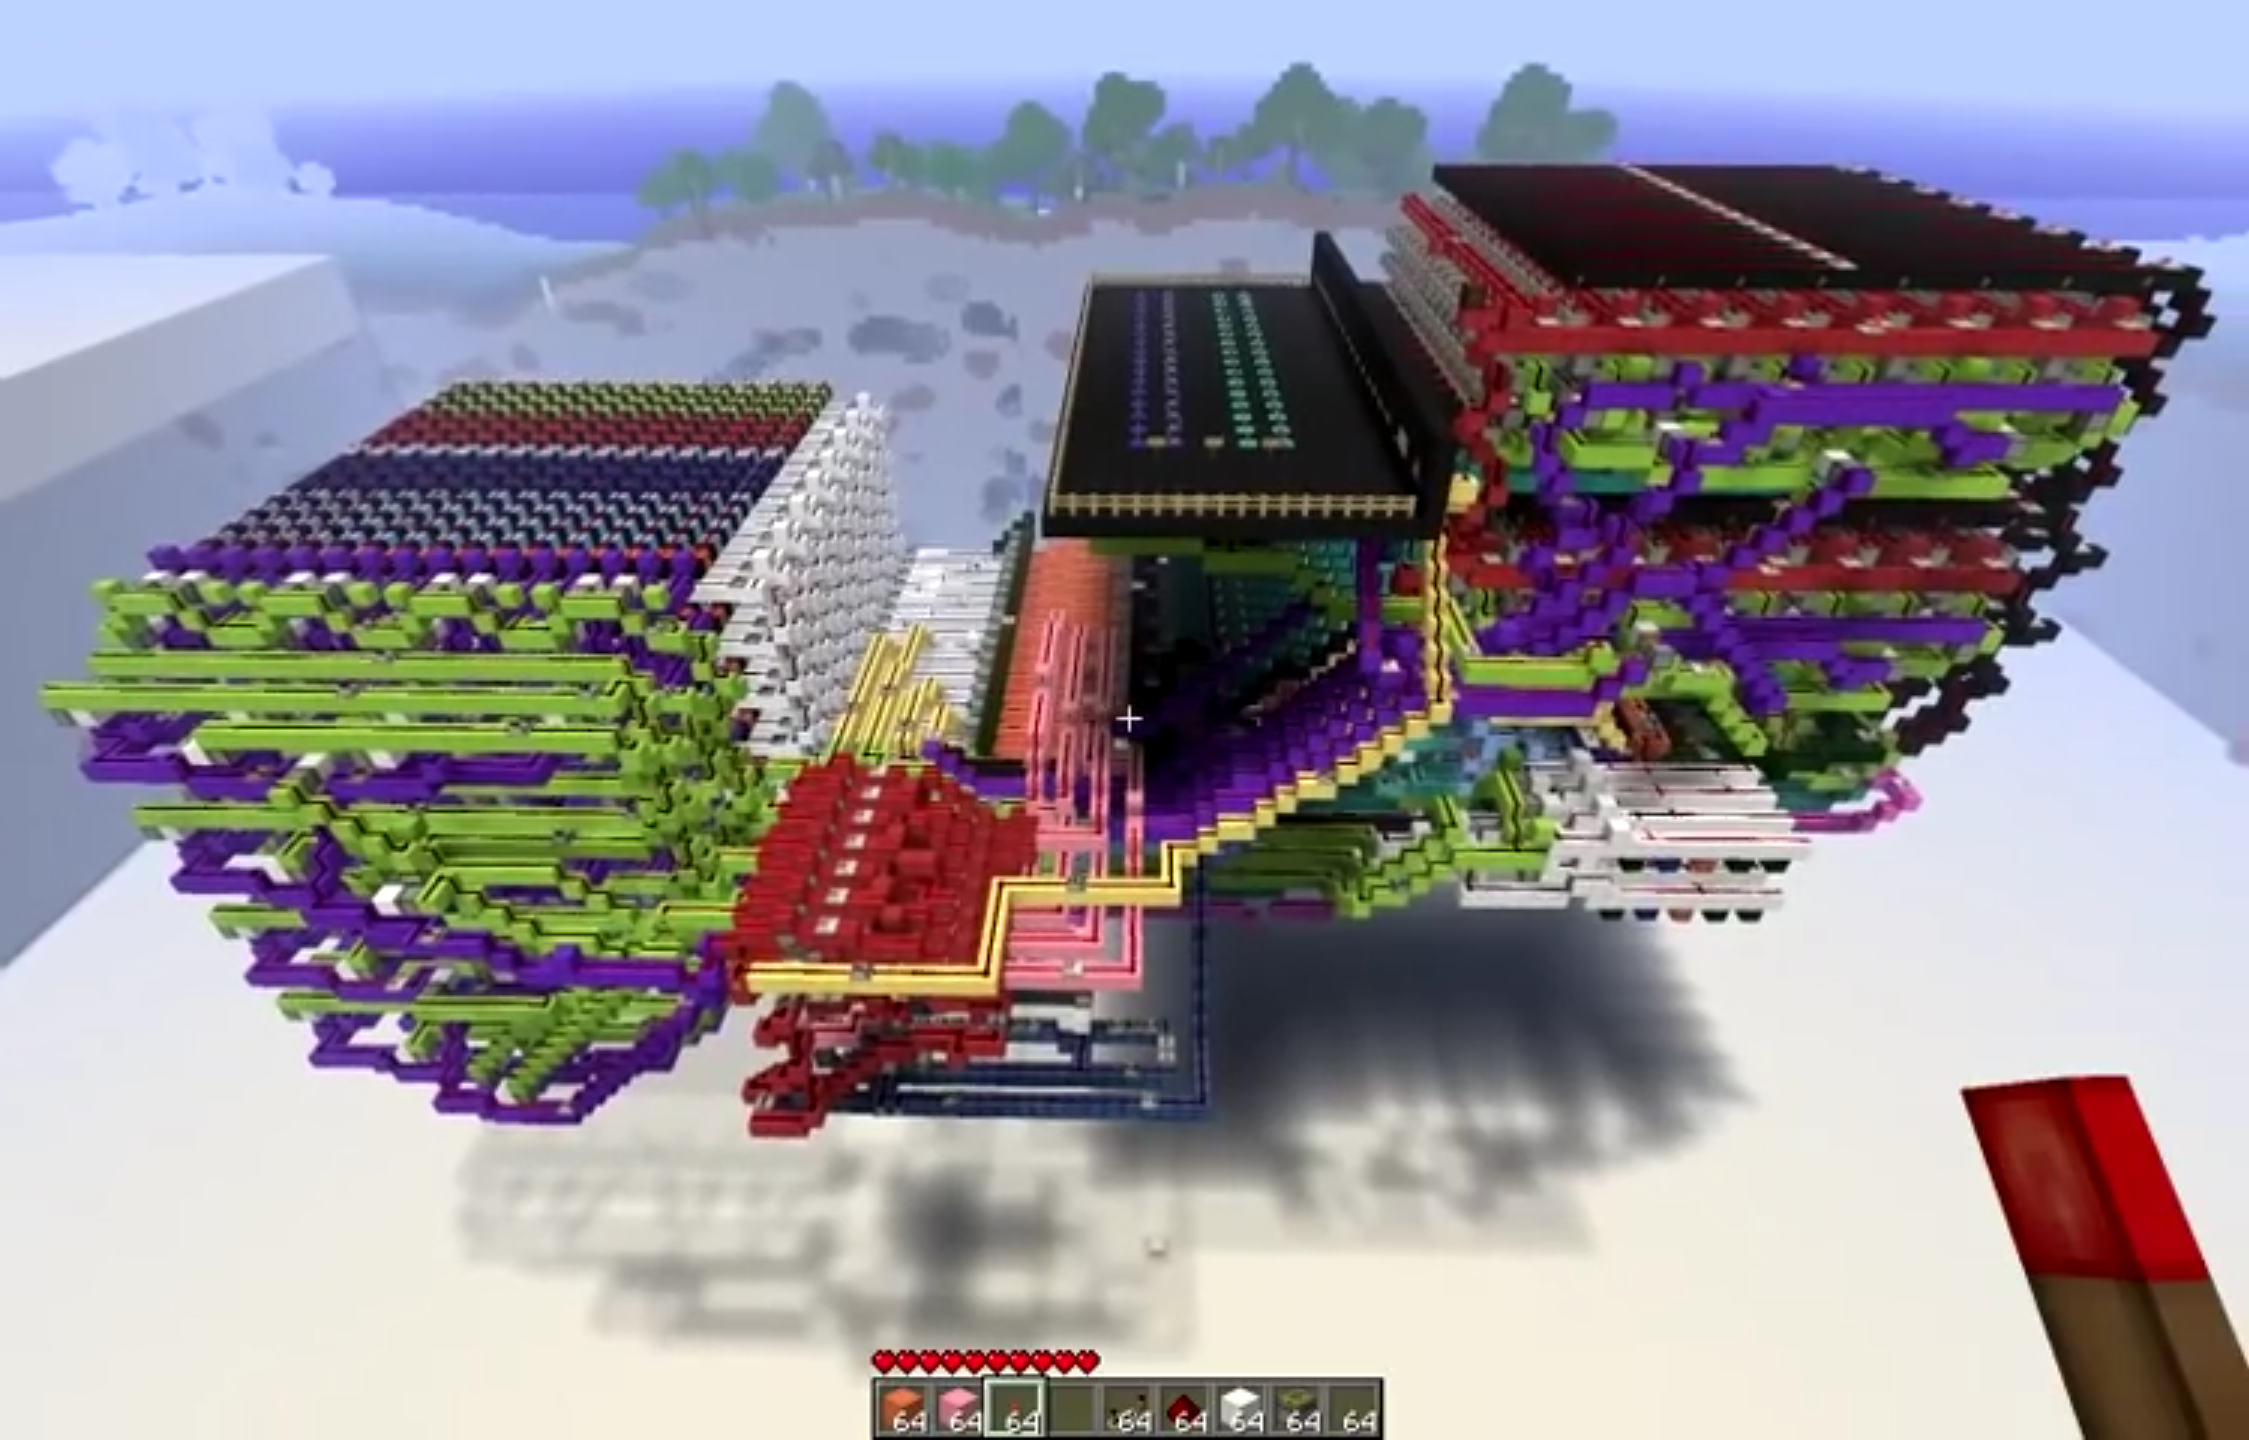
\includegraphics[width=\linewidth]{minecraft.png}
  \caption{Screenshot of a 16 bit computer built in Minecraft by user Ohm.  Full video available on \href{https://www.youtube.com/watch?v=KzrFzkb3A4o}{YouTube}. \textit{Image Credit: Ohm 2011}}
  \label{fig:minecraft}
\end{figure}

The most widely adopted example of discrete design is \href{https://minecraft.net/}{Minecraft}, a PC game that gives players the ability to construct their own worlds from over 100 different block types (Fig \ref{fig:minecraft}).  A subset of these block types form the basis of digital logic in the game and another set of part provide a means of simple 1-bit mechanical actuation \cite{MinecraftWik2016}.  Gameplay and available block types are extendable through various mods and user scripts.
\\

\href{http://golly.sourceforge.net/}{Golly} is a 2D CA simulator originally intended for Conway's game of life, but is extendable to other rulesets.  It implements Gosper's "hashlife" algorithm for optimizing the performance of the simulation \cite{Gosper1984}.  In 2013 Dave Greene Wade published the "Linear Propagator", a self replicating machine designed in Golly using Conway's ruleset \cite{Greene2013a}.  In 2014, Luke Shaeffer implemented a physically universal CA ruleset in Golly, based on interactions between moving particles \cite{Shaffer2014}.\\

\begin{figure}
  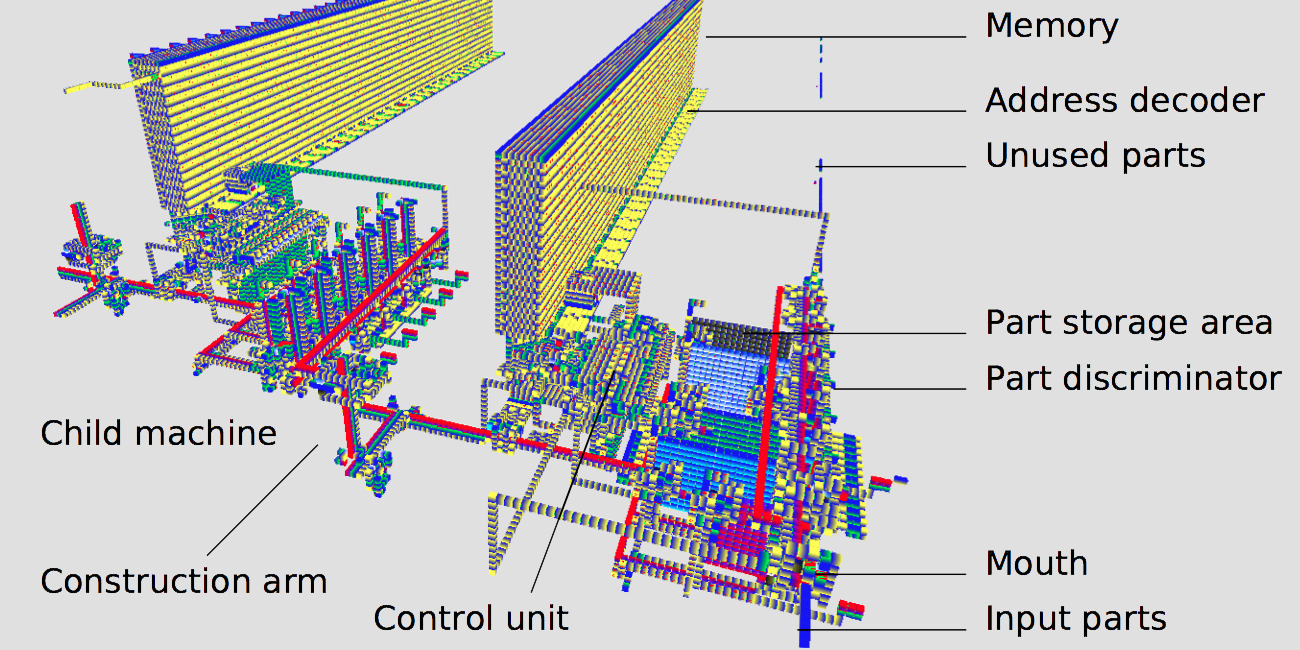
\includegraphics[width=\linewidth]{stevensConstructor.png}
  \caption{A programmable, universal constructor (shown replicating itself) built in CBlock3D by William Stevens from 5040 cells of 6 different types \cite{Stevens2009b}.  Full video of assembly process on  \href{https://www.youtube.com/watch?v=PBXO_6Jn1fs}{YouTube}. \textit{Image Credit: William Stevens 2010}}
  \label{fig:stevensConstructor}
\end{figure}
\href{https://www.youtube.com/watch?feature=player_embedded&v=PBXO_6Jn1fs}{CBlock3D} is a 3D cellular automata environment governed by logical and kinematic rules developed by William Stevens \cite{Stevens2007} \cite{Stevens2009}.  The kinematic simulation in CBlocks3D allows for motions along discrete steps of a regular lattice.  Like Golly, it implements a version of hashlife optimization \cite{Stevens2010} to speed up simulation.  Stevens constructed and simulated a self-replicating machine within this design environment from 5040 cells of 6 distinct types (Fig: \ref{fig:stevensConstructor}) \cite{Stevens2009b}.
\\

\subsection{DNA Origami-Based Tools}

\begin{figure}
  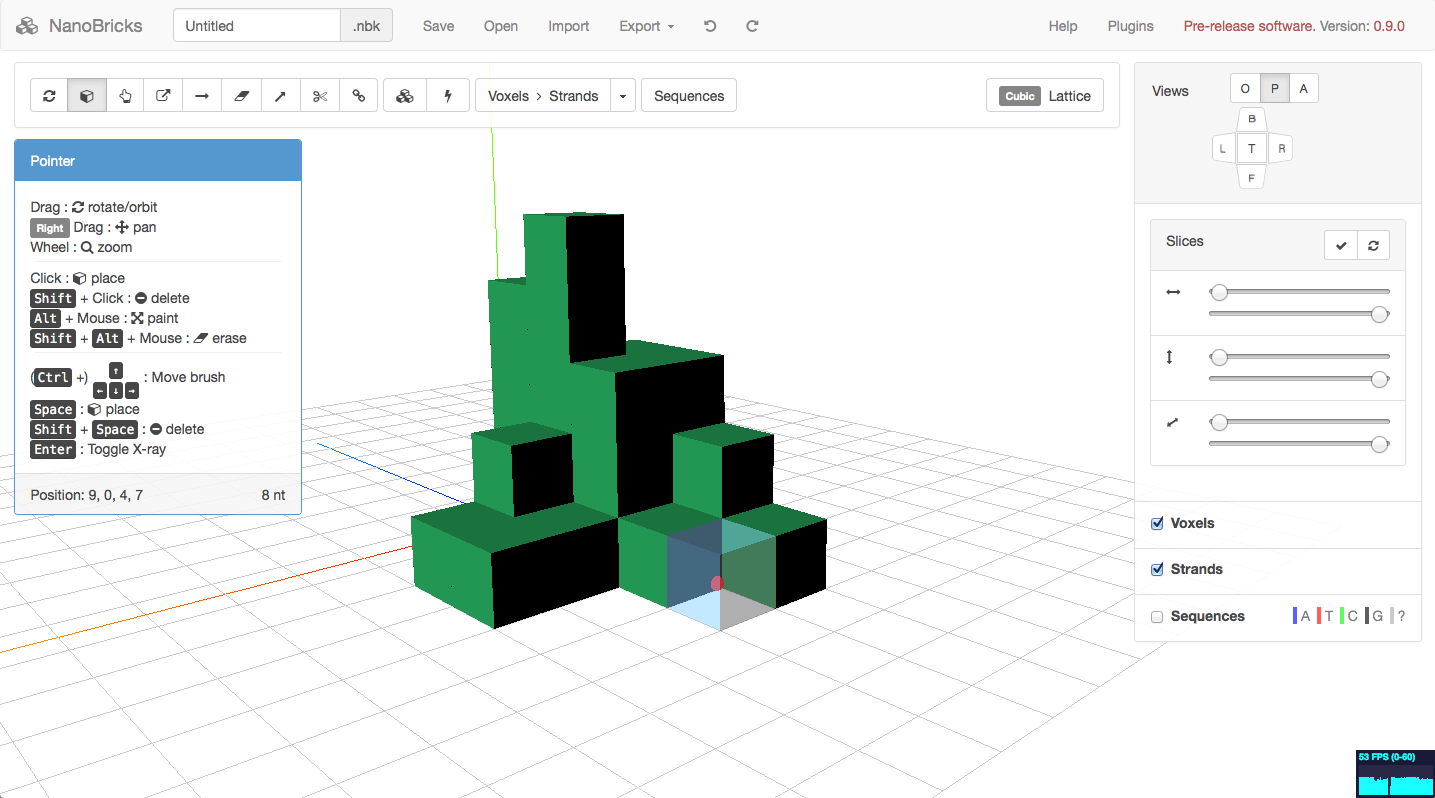
\includegraphics[width=\linewidth]{nanoBricks.png}
  \caption{Screenshot of NanoBricks, a voxel-based design tool for DNA Bricks by the Peng Yin Lab.}
  \label{fig:nanoBricks}
\end{figure}

\href{http://cadnano.org/}{CaDNAno} is a DNA origami design tool originally written by Douglas et al. \cite{Douglas2009}, and later adopted by Autodesk as a plugin for Maya.  It allows users to design 2D and 3D DNA origami structures based on one or several "scaffold" strands folded into a particular shape by many "staple" strands.  Structures are designed on a regular square or honeycomb lattice, though, single nucleotide insertions and deletions can be added to create programmable bending \cite{Dietz2009} \cite{Kim2012}.\\

\href{http://cando-dna-origami.org/}{Cando} is a DNA origami simulation package developed and maintained by Mark Bathe's group at MIT.  It models double stranded DNA as a homogeneous elastic rod with elastic constants and other physical parameters drawn from empirical measurements \cite{Peters2014}.  Crossovers between double stranded segments are modeled as elastic constraints on the rod elements.  Though these crossovers may deform double stranded segments out of a regular lattice configuration (which they are typically designed in) to form complex 3D geometries, simulated CanDo results show good agreement with experimental results \cite{Kim2012a}.  CanDo supports formats from CaDNAno and other DNA design environments.
\\

\href{http://yin.hms.harvard.edu/bricks/try/}{Nanobricks} is a voxel-based design tool for DNA Bricks.  Nanobricks allows a user to design nano-scale structures with voxels on a cubic lattice, and voxel-based designs are converted to sequences and exported as a text file.  Though Nanobricks offers less flexibility than caDNAno (eg it does not allow for out of lattice bending designs), it is significantly easier to design valid structures for a novice user.  Direct integration with CanDo is forthcoming.
\\

\subsection{Physics-Based Tools}

\begin{figure}
  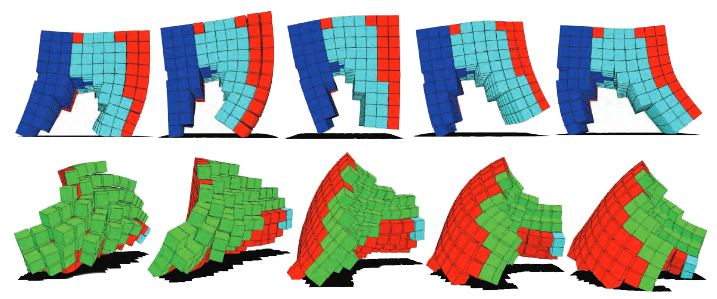
\includegraphics[width=\linewidth]{voxcadWalkers.png}
  \caption{Example gaits of two locomotion robots built from four material types in VoxCAD \cite{Cheney2013b}.  \textit{Image Credit: Cheney et al. 2013}}
  \label{fig:voxcadWalkers}
\end{figure}

\href{http://www.voxcad.com/}{Voxcad} is a physics-based design and dynamic simulation environment by Jonathan Hiller where a user designs virtual soft robots from four block types - two active and two passive \cite{Hiller2014a}.  Though the passive block types descended from a simulation of multimaterial 3D printed voxels, the active block types are not easily fabricated and actuated \cite{Hiller2012} and have not been rigorously evaluated.  Work into the optimization of theoretical locomotion systems in this virtual design space have been explored (Fig: \ref{fig:voxcadWalkers}) \cite{Cheney2013b} \cite{Cheney2013} \cite{Cheney2015}.

}